\documentclass[11pt,compress,t,notes=noshow]{beamer}\usepackage[]{graphicx}\usepackage[]{color}

\makeatletter
\def\maxwidth{ %
  \ifdim\Gin@nat@width>\linewidth
    \linewidth
  \else
    \Gin@nat@width
  \fi
}
\makeatother

\definecolor{fgcolor}{rgb}{0.345, 0.345, 0.345}
\newcommand{\hlnum}[1]{\textcolor[rgb]{0.686,0.059,0.569}{#1}}%
\newcommand{\hlstr}[1]{\textcolor[rgb]{0.192,0.494,0.8}{#1}}%
\newcommand{\hlcom}[1]{\textcolor[rgb]{0.678,0.584,0.686}{\textit{#1}}}%
\newcommand{\hlopt}[1]{\textcolor[rgb]{0,0,0}{#1}}%
\newcommand{\hlstd}[1]{\textcolor[rgb]{0.345,0.345,0.345}{#1}}%
\newcommand{\hlkwa}[1]{\textcolor[rgb]{0.161,0.373,0.58}{\textbf{#1}}}%
\newcommand{\hlkwb}[1]{\textcolor[rgb]{0.69,0.353,0.396}{#1}}%
\newcommand{\hlkwc}[1]{\textcolor[rgb]{0.333,0.667,0.333}{#1}}%
\newcommand{\hlkwd}[1]{\textcolor[rgb]{0.737,0.353,0.396}{\textbf{#1}}}%
\let\hlipl\hlkwb

\usepackage{framed}
\makeatletter
\newenvironment{kframe}{%
 \def\at@end@of@kframe{}%
 \ifinner\ifhmode%
  \def\at@end@of@kframe{\end{minipage}}%
  \begin{minipage}{\columnwidth}%
 \fi\fi%
 \def\FrameCommand##1{\hskip\@totalleftmargin \hskip-\fboxsep
 \colorbox{shadecolor}{##1}\hskip-\fboxsep
     \hskip-\linewidth \hskip-\@totalleftmargin \hskip\columnwidth}%
 \MakeFramed {\advance\hsize-\width
   \@totalleftmargin\z@ \linewidth\hsize
   \@setminipage}}%
 {\par\unskip\endMakeFramed%
 \at@end@of@kframe}
\makeatother

\definecolor{shadecolor}{rgb}{.97, .97, .97}
\definecolor{messagecolor}{rgb}{0, 0, 0}
\definecolor{warningcolor}{rgb}{1, 0, 1}
\definecolor{errorcolor}{rgb}{1, 0, 0}
\definecolor{code}{rgb}{0.97, 0.96, 1.0}
\newenvironment{knitrout}{}{} % an empty environment to be redefined in TeX

\usepackage{alltt}
\usepackage[utf8]{inputenc}
\usepackage[ngerman]{babel}
\usepackage{dsfont}
\usepackage{verbatim}
\usepackage{amsmath}
\usepackage{amsfonts}
\usepackage{mathtools}
\usepackage{csquotes}
\usepackage{cmbright}
\usepackage{multirow}
\usepackage{longtable}
\usepackage{enumerate}
\usepackage[absolute,overlay]{textpos}
\usepackage{psfrag}
\usepackage{algorithm}
\usepackage{algpseudocode}
\usepackage{eqnarray}
\usepackage{bytefield}
\usepackage{animate}
\usepackage{tikz}
\usetikzlibrary{shapes,matrix,positioning,chains,arrows,shadows,decorations.pathmorphing,fit,backgrounds}
\usepackage{adjustbox}
\usepackage{colortbl}
\usepackage{tabularx} % for tables (incl. \hline)
\usepackage{arydshln} % Load after array, longtable, colortab and/or colortbl , otherwise problems with \hline in tabular env
\usepackage{etex} %increase registers for \dimenS to more than 256, otherwise we get "No room for a new \dimen"
\usepackage{graphicx}
\usepackage{booktabs} %used in epr lectures
\usepackage{bm} % bold greek letters
\usepackage{hyperref} % url citing
\usepackage{blkarray} % block arrays
\usepackage{listings} % block of code
\usepackage{xcolor} %colored math symbols
\usepackage{pgffor}
\usepackage{verbatimbox}
\usepackage{xcolor}

%some colors
\definecolor{checkgreen}{HTML}{18A126}
\definecolor{errorred}{HTML}{FF0000}
\definecolor{blockbg}{HTML}{F7F7F7}
\definecolor{gray}{HTML}{A0A0A0}

% basic latex stuff
\newcommand{\col}{\par\colorbox{code}{\parbox{\textwidth}{\theverbbox}}\par}
\newcommand{\eg}{e.\,g.\xspace} %for example
\newcommand{\ie}{i.\,e.\xspace} %that is to say...
\newcommand{\pkg}[1]{{\fontseries{b}\selectfont #1}} %fontstyle for R packages
\newcommand{\lz}{\vspace{0.5cm}} %vertical space
\newcommand{\oneliner}[1] % Oneliner for important statements
{\begin{block}{}\begin{center}\begin{Large}#1\end{Large}\end{center}\end{block}}
\def\SpAr{\quad \Rightarrow \quad}

%new environments
\newenvironment{vbframe}  %frame with breaks and verbatim
{
 \begin{frame}[containsverbatim,allowframebreaks]
}
{
\end{frame}
}

\newenvironment{vframe}  %frame with verbatim without breaks (to avoid numbering one slided frames)
{
 \begin{frame}[containsverbatim]
}
{
\end{frame}
}

\newenvironment{blocki}[1]   % itemize block
{
 \begin{block}{#1}\begin{itemize}
}
{
\end{itemize}\end{block}
}

\newenvironment{fragileframe}[2]{  %fragile frame with framebreaks
\begin{frame}[allowframebreaks, fragile, environment = fragileframe]
\frametitle{#1}
#2}
{\end{frame}}

\newcommand{\myframe}[2]{  %short for frame with framebreaks
\begin{frame}[allowframebreaks]
\frametitle{#1}
#2
\end{frame}}

\usepackage{../../style/lmu-lecture}

\let\code=\texttt
\let\proglang=\textsf

\setkeys{Gin}{width=0.9\textwidth}

\usepackage{tikz}
\usetikzlibrary{shapes,arrows,snakes, calc}

% Define block styles
\tikzstyle{decision} = [diamond, draw, text width=6em, text badly centered, node distance=4cm, inner sep=0pt]
\tikzstyle{decision2} = [diamond, draw, fill=customgreen!35, text width=6em, text badly centered, node distance=4cm, inner sep=0pt]

\tikzstyle{block} = [rectangle, draw, text width=14em, text centered, rounded corners, node distance=3cm, minimum height=4em]
\tikzstyle{line} = [draw, -latex']
\tikzstyle{cloud} = [draw, ellipse, node distance=3cm, minimum height=2em]

\title{Introduction to Deep Learning}
\author{Bernd Bischl}
\institute{Department of Statistics -- LMU Munich}
\date{WS 2021/2022}

\setbeamertemplate{frametitle}{\expandafter\uppercase\expandafter\insertframetitle}

\IfFileExists{upquote.sty}{\usepackage{upquote}}{}
\input{../../latex-math/basic-math}
\input{../../latex-math/basic-ml}
\input{../../latex-math/ml-nn}

\begin{document}

\lecturechapter{3}{Basic Regularization}
\lecture{Basic Regularization}
%%%%%%%%%%%%%%%%%%%%%%%%%%%%%%%%%%%%%%%%%%%%%%%%%%%%%%%%%%%%%%%%%%

\begin{frame} {Regularization}
\begin{itemize}
\item Any technique that is designed to reduce the test error possibly at the expense of increased training error can be considered a form of regularization.
\item Regularization is important in DL because NNs can have extremely high capacity (millions of parameters).
\end{itemize}
\end{frame}
%%%%%%%%%%%%%%%%%%%%%%%%%%%%%%%%%%%%%%%%%%%%%%%%%%%%%%%%%%%%%%%%%%

\begin{vbframe}{Revision: Regularized Risk Minimization}
\begin{itemize}
\item The goal of regularized risk minimization is to penalize the complexity of the model to minimize the chances of overfitting.
\item By adding a parameter norm penalty term \(J(\thetab)\) to the empirical risk $\risket$ we obtain a regularized cost function:
$$\riskrt = \risket + \lambda \text{\(J(\thetab)\)}$$
with hyperparamater $\lambda \in [0, \infty)$, that weights the penalty term, relative to the unconstrained objective function $\risket$.
\item Therefore, instead of pure \textbf{empirical risk minimization}, we add a penalty
for complex (read: large) parameters \(\thetab\).
\item Declaring $\lambda = 0$ obviously results in no penalization.
\item We can choose between different parameter norm penalties \(J(\thetab)\).
\item In general, we do not penalize the bias.
\end{itemize}
\end{vbframe}
%%%%%%%%%%%%%%%%%%%%%%%%%%%%%%%%%%%%%%%%%%%%%%%%%%%%%%%%%%%%%%%%%%

\begin{vbframe}{L2-regularization / Weight decay}
Let us optimize the L2-regularized risk of a model $\fxt$
\[\min_{\thetab} \riskrt = \min_{\thetab} \risket + \frac{\lambda}{2} \|\thetab\|^2_2\]
by gradient descent. The gradient is
\[\nabla \riskrt = \nabla \risket + \lambda \thetab.\]
We iteratively update $\thetab$ by step size \(\alpha\) times the
negative gradient
\[\thetab^{[\text{new}]} = \thetab^{[\text{old}]} - \alpha \left(\nabla \risket + \lambda \thetab^{[\text{old}]}\right) =
\thetab^{[\text{old}]} (1 - \alpha \lambda) - \alpha \nabla \risket\]
$\to$ The term \(\lambda \thetab^{[old]}\) causes the parameter
(\textbf{weight}) to \textbf{decay} in proportion to its size (which gives rise to the name). 
\framebreak
%%%%%%%%%%%%%%%%%%%%%%%%%%%%%%%%%%%%%%%%%%%%%%%%%%%%%%%%%%%%%%%%%%

Weight decay can be interpreted \textbf{geometrically}. 
\lz 
Let us make a quadratic approximation of the unregularized objective $\risket$ in the neighborhood of its minimizer $\thetah$,  
$$ \mathcal{\tilde R}_{\text{emp}}(\thetab)= \mathcal{R}_{\text{emp}}(\thetah) + \nabla \mathcal{R}_{\text{emp}}(\thetah)\cdot(\thetab - \thetah) + \ \frac{1}{2} (\thetab - \thetah)^T \bm{H} (\thetab - \thetah), $$
where $\bm{H}$ is the Hessian matrix of $\risket$ w.r.t. $\thetab$ evaluated at $\thetah$. 
\lz
Because $\thetah = \argmin_{\thetab}\risket$,
\begin{itemize}
\item the first order term is 0 in the expression above because the gradient is $0$, and,
\item $\bm{H}$ is positive semidefinite.
\end{itemize}
\lz
\tiny{Source: Goodfellow et al. (2016), ch. 7}
\framebreak
%%%%%%%%%%%%%%%%%%%%%%%%%%%%%%%%%%%%%%%%%%%%%%%%%%%%%%%%%%%%%%%%%%

\normalsize
The minimum of $\mathcal{\tilde R}_{\text{emp}}(\thetab)$ occurs where $\nabla_{\thetab}\mathcal{\tilde R}_{\text{emp}}(\thetab) = \bm{H}(\thetab - \thetah)$ is $0$.
\lz
Adding the weight decay gradient $\lambda \thetab$, we get the regularized version of $\mathcal{\tilde R}_{\text{emp}}(\thetab)$. We solve it for the minimizer $\hat{\thetab}_{\text{Ridge}}$:
\begin{gather*}
\lambda \thetab + \bm{H}(\thetab - \thetah) = 0\\
(\bm{H} + \lambda \id) \thetab = \bm{H} \thetah \\
\hat{\thetab}_{\text{Ridge}} = (\bm{H} + \lambda \id)^{-1}\bm{H} \thetah
\end{gather*}
where $\id$ is the identity matrix.
\lz
As $\lambda$ approaches $0$, the regularized solution $\hat{\thetab}_{\text{Ridge}}$ approaches $\thetah$. What happens as $\lambda$ grows?
\framebreak
%%%%%%%%%%%%%%%%%%%%%%%%%%%%%%%%%%%%%%%%%%%%%%%%%%%%%%%%%%%%%%%%%%

\begin{itemize}
\item Because $\bm{H}$ is a real symmetric matrix, it can be decomposed as $\bm{H} = \bm{Q} \bm{\Sigma} \bm{Q}^\top$ where $\bm{\Sigma}$ is a diagonal matrix of eigenvalues and $\bm{Q}$ is an orthonormal basis of eigenvectors.
\item Rewriting the equation on the previous slide using the eigendecomposition above,

\begin{equation*}
\begin{aligned} 
\hat{\thetab}_{\text{Ridge}} &=\left(\bm{Q} \bm{\Sigma} \bm{Q}^{\top}+\lambda \id\right)^{-1} \bm{Q} \bm{\Sigma} \bm{Q}^{\top} \thetah \\ 
              &=\left[\bm{Q}(\bm{\Sigma}+\lambda \id) \bm{Q}^{\top}\right]^{-1} \bm{Q} \bm{\Sigma} \bm{Q}^{\top} \thetah \\ 
              &=\bm{Q}(\bm{\Sigma} + \lambda \id)^{-1} \bm{\Sigma} \bm{Q}^{\top} \thetah 
\end{aligned}
\end{equation*}
\item Therefore, the weight decay rescales $\thetah$ along the axes defined by the eigenvectors of $\bm{H}$. The component of $\thetah$ that is aligned with the $i$-th eigenvector of $\bm{H}$ is rescaled by a factor of $\frac{\sigma_i}{\sigma_i + \lambda}$, where $\sigma_i$ is the corresponding eigenvalue.
\framebreak
%%%%%%%%%%%%%%%%%%%%%%%%%%%%%%%%%%%%%%%%%%%%%%%%%%%%%%%%%%%%%%%%%%

  \item Along directions where the eigenvalues of $\bm{H}$ are relatively large, for example, where $\sigma_i >> \lambda$, the effect of regularization is quite small.
  \item On the other hand, components with $\sigma_i << \lambda$ will be shrunk to have nearly zero magnitude.
  \item In other words, only directions along which the parameters contribute significantly to reducing the objective function are preserved relatively intact.
  \item In the other directions, a small eigenvalue of the Hessian means that moving in this direction will not significantly increase the gradient. For such unimportant directions, the corresponding components of $\thetab$ are decayed away.
  \end{itemize}
\framebreak
%%%%%%%%%%%%%%%%%%%%%%%%%%%%%%%%%%%%%%%%%%%%%%%%%%%%%%%%%%%%%%%%%%

\begin{figure}
\centering
\scalebox{0.36}{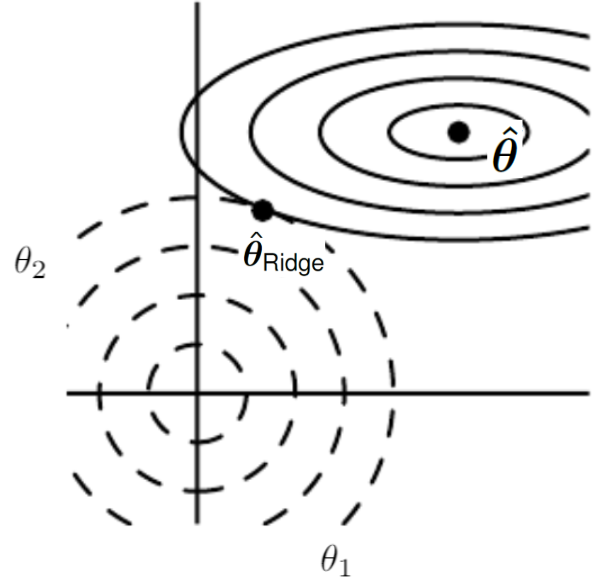
\includegraphics{figure/wt_decay_hat.png}}
\tiny{\\ Credit: Goodfellow et al. (2016), ch. 7}
\caption{\footnotesize The solid ellipses represent the contours of the unregularized objective and the dashed circles represent the contours of the L2 penalty. At $\hat{\thetab}_{\text{Ridge}}$, the competing objectives reach an equilibrium.}
\end{figure}
\small
In the first dimension, the eigenvalue of the Hessian of $\risket$ is small. The objective function does not increase much when moving horizontally away from $\thetah$. Therefore, the regularizer has a strong effect on this axis and $\theta_1$ is pulled close to zero.
\framebreak
%%%%%%%%%%%%%%%%%%%%%%%%%%%%%%%%%%%%%%%%%%%%%%%%%%%%%%%%%%%%%%%%%%

\begin{figure}
\centering
\scalebox{0.36}{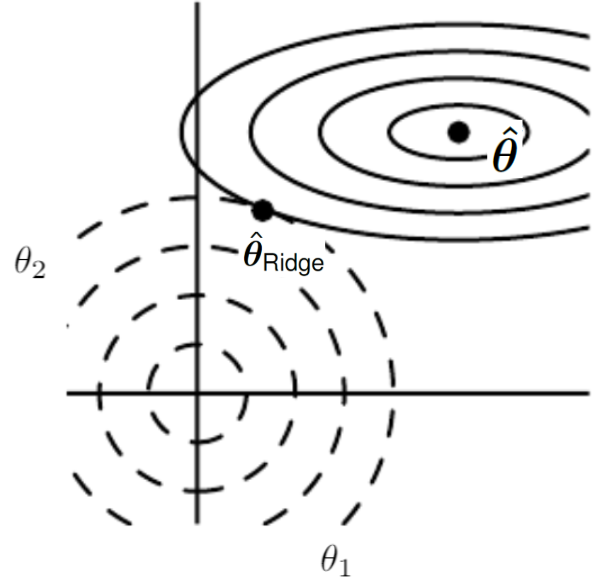
\includegraphics{figure/wt_decay_hat.png}}
\tiny{\\ Credit: Goodfellow et al. (2016), ch. 7}
\caption{\footnotesize The solid ellipses represent the contours of the unregularized objective and the dashed circles represent the contours of the L2 penalty. At $\hat{\thetab}_{\text{Ridge}}$, the competing objectives reach an equilibrium.}
\end{figure}
In the second dimension, the corresponding eigenvalue is large indicating high curvature. The objective function is very sensitive to movement along this axis and, as a result, the position of $\theta_2$ is less affected by the regularization.
\end{vbframe}
%%%%%%%%%%%%%%%%%%%%%%%%%%%%%%%%%%%%%%%%%%%%%%%%%%%%%%%%%%%%%%%%%%

\begin{vbframe} {L1-Regularization}
\begin{itemize}
\item The L1-regularized risk of a model $\fxt$ is
\[\min_{\thetab} \riskrt = \risket + \lambda ||\thetab||_1\] 
and the (sub-)gradient is:
$$\nabla_{\theta} \mathcal{R}_{\text{reg}}(\thetab) = \lambda \sign(\thetab) + \nabla_{\theta} \risket$$
\item Note that, unlike in the case of L2, the contribution of the L1 penalty to the gradient doesn't scale linearly with each $\theta_i$. Instead, it is a constant factor with a sign equal to $\sign(\theta_i)$.
\item Let us now make a quadratic approximation of $\mathcal{R}_{\text{emp}}(\thetab)$. To get a clean algebraic expression, we assume the Hessian of $\mathcal{R}_{\text{emp}}(\thetab)$ is diagonal, i.e. $\bm{H} = \text{diag}([H_{1,1}, \ldots , H_{n,n}])$, where each $H_{i,i} > 0$.
\item This assumption holds, for example, if the input features for a linear regression task have been decorrelated using PCA.
\end{itemize}
\framebreak
%%%%%%%%%%%%%%%%%%%%%%%%%%%%%%%%%%%%%%%%%%%%%%%%%%%%%%%%%%%%%%%%%%

\begin{itemize}
\item The quadratic approximation of $\mathcal{R}_{\text{reg}}(\thetab)$ decomposes into a sum over the parameters:
  $$\mathcal{\tilde R}_{\text{reg}}(\thetab) = \mathcal{R}_{\text{emp}}(\thetah) + \sum_i \left[ \frac{1}{2} H_{i,i} (\theta_i - \hat{\theta}_i)^2 \right] + \sum_i \lambda |\theta_i|$$
  where $\thetah$ is the minimizer of the unregularized risk $\risket$.
\item The problem of minimizing this approximate cost function has an analytical solution (for each dimension $i$), with the following form:
$$\hat{\theta}_{\text{Lasso},i} = \sign(\hat{\theta}_i) \max \left\{ |\hat{\theta}_i| - \frac{\lambda}{H_{i,i}},0 \right\}$$
\item If  $0 < \hat{\theta}_i \leq \frac{\lambda}{H_{i,i}}$, the optimal value of $\theta_i$ (for the regularized risk) is $0$ because the contribution of  $\risket$ to $\riskrt$ is overwhelmed by the L1 penalty, which forces it to be $0$.
\item If $0 < \frac{\lambda}{H_{i,i}} < \hat{\theta}_i$, the $L1$ penalty shifts the optimal value of $\theta_i$ toward 0 by the amount $\frac{\lambda}{H_{i,i}}$.
\item A similar argument applies when $\hat{\theta}_i < 0$. 
\item Therefore, the L1 penalty induces sparsity in the parameter vector.
\end{itemize}
\end{vbframe}
%%%%%%%%%%%%%%%%%%%%%%%%%%%%%%%%%%%%%%%%%%%%%%%%%%%%%%%%%%%%%%%%%%

\begin{frame}{Equivalence to Constrained Optimization}
Norm penalties can be interpreted as imposing a constraint on the weights. One can show that 
 $$\argmin_{\theta} \risket + \lambda \text{\(J(\thetab)\)}$$
 is equvilalent to
 \begin{align*}
 & \argmin_{\thetab}  \risket \\
  &\text{subject to \;\;\;}  J(\thetab) \leq k
 \end{align*}
 for some value $k$ that depends on $\lambda$ the nature of 
 $\risket$.\\[0.3cm]
 \scriptsize{(Goodfellow et al. (2016), ch. 7.2)}
\end{frame}
%%%%%%%%%%%%%%%%%%%%%%%%%%%%%%%%%%%%%%%%%%%%%%%%%%%%%%%%%%%%%%%%%%

\begin{vbframe}{Example: Weight decay}
\begin{minipage}{0.45\textwidth}
\begin{itemize}
\item We fit the huge neural network on the right side on a smaller fraction of MNIST (5000 train and 1000 test observations)
\item Weight decay: $\lambda \in (10^{-2}, 10^{-3}, 10^{-4}, 10^{-5}, 0)$
\end{itemize}
\end{minipage}
\begin{minipage}{0.45\textwidth}
\begin{figure}
\centering
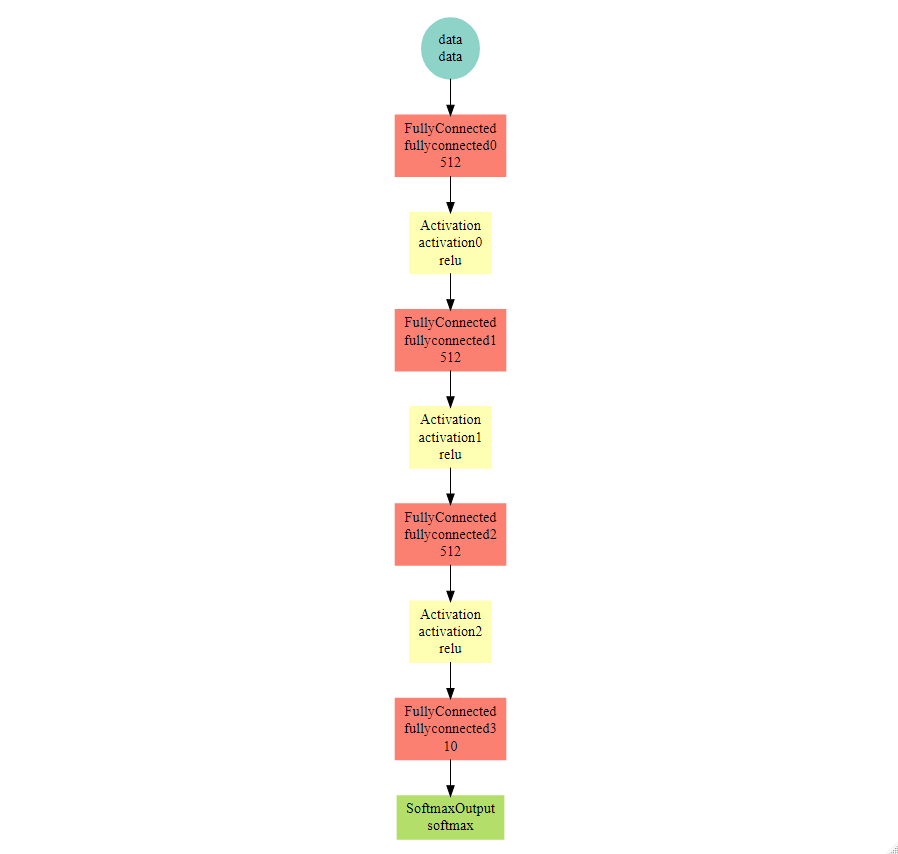
\includegraphics[width=8.7cm]{figure/mxnet_graph_decay.png}
\end{figure}
\end{minipage}
\framebreak
%%%%%%%%%%%%%%%%%%%%%%%%%%%%%%%%%%%%%%%%%%%%%%%%%%%%%%%%%%%%%%%%%%

\begin{figure}
\centering
\scalebox{1}{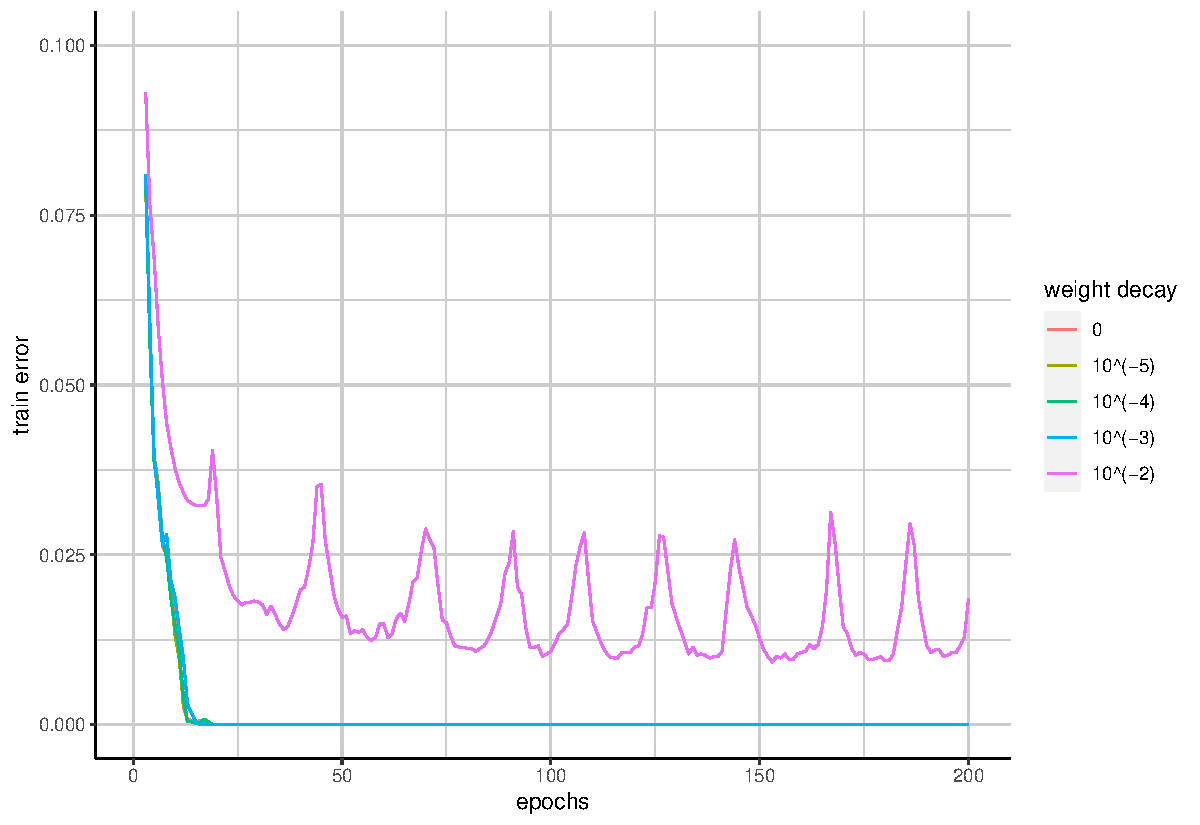
\includegraphics{figure_man/weight_decay1.pdf}}
\\
A high weight decay of $10^{-2}$ leads to a high error on the training data.
\end{figure}

\framebreak
%%%%%%%%%%%%%%%%%%%%%%%%%%%%%%%%%%%%%%%%%%%%%%%%%%%%%%%%%%%%%%%%%%

\begin{figure}
\centering
\scalebox{1}{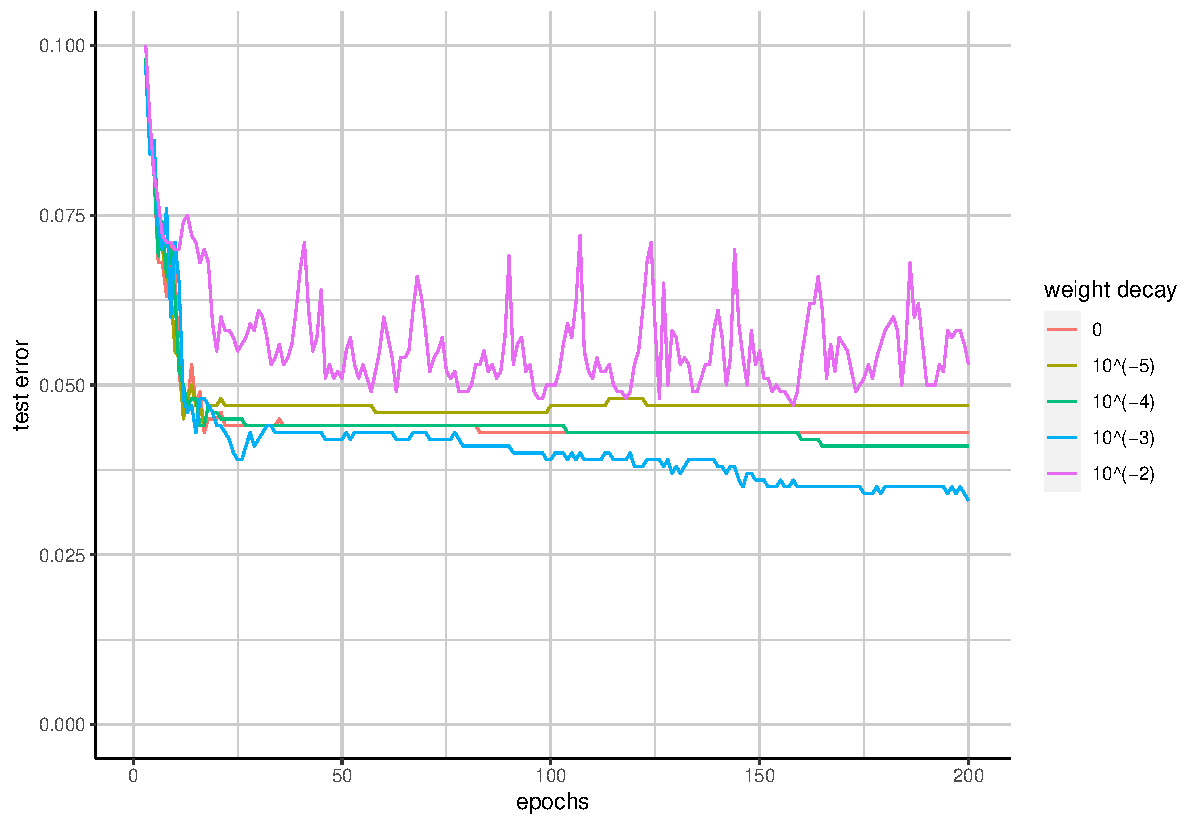
\includegraphics{figure_man/weight_decay2.pdf}}
\\
Second strongest weight decay leads to the best result on the test data.
\end{figure}
\end{vbframe}
  
%%%%%%%%%%%%%%%%%%%%%%%%%%%%%%%%%%%%%%%%%%%%%%%%%%%%%%%%%%%%%%%%%%
\begin{frame}{Tensorflow Playground}
\begin{figure}
\centering
\scalebox{1}{
\includegraphics{figure/tensorflow_playground.png}}
  \end{figure}
  \scriptsize
  \url{https://playground.tensorflow.org/}
\end{frame}

\begin{frame}{Tensorflow Playground - Exercise}
  \begin{figure}
    \centering
      \scalebox{1}{
\includegraphics{figure/tensorflow_exercise.png}}
  \end{figure}
  \scriptsize
  \url{https://developers.google.com/machine-learning/crash-course/regularization-for-simplicity/playground-exercise-examining-l2-regularization}
\end{frame}

%%%%%%%%%%%%%%%%%%%%%%%%%%%%%%%%%%%%%%%%%%%%%%%%%%%%%%%%%%%%%%%%%%

\endlecture
\end{document}